\chapter{Servizio Cittadino}

Il servizio cittadino (\emph{City Service} o CS) è il cuore dell'architettura software e supporta le interazioni tra gli EV e la Smart Grid. Lo scambio di informazioni avviene tramite il \emph{City SIB} con la struttura dei messaggi definita all'interno dell'Ontologia. 

\section{Architettura}

Il CS era già stato implementato da Federico Montori nel progetto precedente. Ho deciso di riscriverlo puntando ad una maggiore modularità e riusabilità. Ho quindi creato libreria di cui ho già trattato in Sez. \ref{subsec:ioe-lib} condivisa tra il servizio cittadino e l'applicazione mobile. La libreria fornisce i servizi di base per l'accesso al SIB con un approccio \emph{Object Oriented} ai dati in essa contenuti. Questa scelta progettuale si rifà ai principi di Ingegneria del Software \emph{High Cohesion} e \emph{Low Coupling} \cite{larcab2005}

\section{La comunicazione con il City Service}\label{sec:protocol}

In questa sezione si analizzano in dettaglio le modalità di comunicazione da e verso il servizio cittadino. Per ogni operazione esiste un protocollo basato su scambio di messaggi la cui struttura è definita mediante classi dell'ontologia. Attualmente le uniche operazioni supportate sono la richiesta di prenotazione e la richiesta di ritiro di prenotazione.

Lo scambio dei messaggi è implementato tramite il meccanismo delle Subscription messo a disposizione dal SIB. Questo comporta che i messaggi si scrivano sul SIB cittadino che manda una notifica al KP sottoscritto a quella particolare modifica. Ne consegue un protocollo di comunicazione asincrono.

\subsection{Protocollo di richiesta di prenotazione}

Descriverò i passaggi necessari al completamento del protocollo di richiesta di prenotazione con particolare attenzione ai messaggi vengono scambiati. Il fine della prenotazione è la certezza di trovare l'EVSE libero quando andremo a caricarci. Come già detto in precedenza, i tempi di ricarica per i veicoli elettrici possono essere molto lunghi. È quindi necessario dare all'utente la certezza che potrà ricaricare il suo veicolo senza il rischio di terminare la carica della batteria.

\begin{enumerate}[label=\textbf{\arabic*}]
	\item \textbf{Richiesta di Prenotazione}: quando l'utente necessita di fare una ricarica inserisce una richiesta nel SIB. La richiesta è descritta dalla classe dell'ontologia \code{ioe:ChargeRequest}.
	\item \textbf{Risposta da parte del City Service}: il servizio cittadino è sottoscritto all'inserimento di nuove istanze di \code{ioe:ChargeRequest}. Quindi quando si inserisce la richiesta, il CS riceve una notifica che ne contiene l'URI dal quale può ricavare i parametri che la compongono. A questo punto viene creata una lista di opzioni di ricarica conformi alla richiesta dell'utente compatibilmente con la disponibilità degli EVSE. Le opzioni di ricarica sono classi di tipo \code{ioe:ChargeOption} e vengono inserite dentro a una classe di tipo \code{ioe:ChargeResponse}.
	\item \label{item:confirmByUser} \textbf{Conferma da parte dell'utente}: L'utente che è sottoscritto all'inserimento di nuove istanze della classe \code{ioe:ChargeResponse} viene avvisato dal SIB quando il CS inserisce la risposta. Le opzioni di ricarica vengono analizzate dall'utente che sceglierà quella più consona alle sue esigenze. La scelta viene notificata al sistema tramite inserimento di una tripla così formata: \code{[ioe:chargeOptURI ioe:confirmByUser "true"]} presupponendo che \code{ioe:chargeOptURI} sia un istanza di \\ \code{ioe:ChargeOption}.
	\item \textbf{Conferma da parte del City Service}: Il servizio cittadino, iscritto all'inserimento di triple aventi come predicato \code{ioe:confirmByUser}, verifica se l'opzione selezionata è ancora disponibile e in tal caso inserisce la tripla:\code{[ioe:chargeOptURI ioe:confirmBySystem "true"]}. 
	\item \textbf{Acknowledgment da parte dell'utente}: L'utente riceve la notifica della conferma da parte di CS. Se l'opzione è confermata il CS invia una tripla di Acknowledgment \code{[ioe:userURI ioe:ackByUser "true"]}. Altrimenti può provare con un altra opzione e il protocollo riprende dal punto ~\ref{item:confirmByUser}.
	\item \textbf{Creazione Prenotazione}: Il CS, ricevuto l'acknowledgment dall'utente, ``blocca'' l'EVSE nella finestra di tempo richiesta creando un istanza della classe \code{ioe:Reservation}. Inoltre cancella dal SIB tutte le triple necessarie allo svolgimento del protocollo che, una volta terminato, diventano inutili.
\end{enumerate}

\section{Il Protocollo di rimozione di una prenotazione}

Una volta completata la procedura di prenotazione l'EVSE diventa inagibile nella finestra di tempo richiesta dall'utente. Per ritirare la prenotazione l'utente deve inviare una richiesta al CS. Attualmente il servizio cittadino rimuove semplicemente dal SIB i dati relativi alla prenotazione rendendo nuovamente disponibile la ricarica. In futuro il servizio potrà stabilire, in base a regole dettate dai gestori della rete elettrica, se accettare o meno la richiesta ed eventualmente accreditare una penale all'utente.

Come nel caso precedente il protocollo si basa su cambio di messaggi.

\begin{enumerate}
	\item \textbf{Richiesta ritiro Prenotazione}: l'utente inserisce nel SIB cittadino un istanza della classe \code{ioe:ReservationRetire} 
	\item \textbf{Ritiro della Prenotazione}: il CS, ovviamente era sottoscritto alla creazione di nuove istanze di \code{ioe:ReservationRetire}, provvede a rimuovere dal SIB le triple relative alla Prenotazione.
	\item \textbf{Notifica avvenuta cancellazione}: attualmente l'utente per accertarsi dell'avvenuta cancellazione deve sottoscriversi ai cambiamenti relativi all'URI della prenotazione che sta cancellando.
\end{enumerate}

\section{Implementazione}\label{sec:impl}

In questa sezione discuteremo i dettagli implementativi del \emph{City Service}, dalle tecnologie usate alle scelte architetturali. Principalmente il servizio cittadino deve essere altamente performante in quanto, una vota a regime, deve essere in grado di soddisfare le richieste di centinaia se non migliaia di utenti. Contemporaneamente bisogna controllare che l'elevato parallelismo di thread gestiti dal CS non intacchi l'integrità dei dati residenti sul SIB cittadino per evitare ad esempio che due persone che prenotano nello stesso momento e nello stesso EVSE riescano entrambe a completare la procedura di prenotazione. 

Il servizio è scritto interamente in Java. Questo lo rende multi piattaforma, facile da \emph{debuggare} e sopratutto consente l'uso di utilità estremamente versatili riguardo al multi-threading rese disponibili dal linguaggio. Inoltre permette di accedere alla moltitudine di librerie scritte per le più disparate necessità. Tra queste troviamo \emph{log4j}, un robusto quanto versatile sistema di logging che permette di tenere costantemente sotto controllo l'esecuzione del servizio con vari gradi di granularità del log.

Per rendere il servizio più performante possibile si sono adottate tecniche di programmazione quali: pool di oggetti, pool di thread, e caching delle risorse.

\subsection{Pool Di Oggetti}

Per effettuare le connessioni al SIB cittadino è necessario istanziare oggetti di tipo \code{KpConnector}. Inoltre per effettuare il parsing delle risposte alle sottoscrizioni sono necessari oggetti di tipo \code{SSAP_XMLTools} forniti dalla libreria JavaKPI. Come anticipato nella Sez. \ref{sec:impl} il CS deve supportare connessioni multiple simultanee, ognuna delle quali dialogante con il SIB. Dal momento che ne la libreria JavaKPI ne wrapper da me creato sono thread-safe, è necessario istanziare un oggetto \code{KpConnector} per ogni connessione insieme a uno di tipo \code{SSAP_XMLTools} per \emph{parsare} i risultati delle sottoscrizioni.

Per evitare che all'avvio di ogni connessione venisse creato un oggetto \code{KpConnector}, operazione assai onerosa, ho optato per la tecnica dei pool di oggetti. Questa consiste nel creare un numero sufficiente di istanziare oggetti all'inizio dell'applicazione e quando ne serve uno lo si chiede al pool che lo fornisce nel tempo di una \emph{chiamata a metodo}. Terminato l'uso dell'oggetto lo si restituisce al pool che lo renderà disponibile ad un altro richiedente.
Cosi si evita il delay necessario a instanziare una connessione con il SIB ogni volta che si esegue una richiesta al CS.

Aggiungo che, viste le ottimizzazioni delle moderne \emph{Java Virtual Machine} e dei \emph{Garbage Collector} per quanto riguarda gli oggetti con breve durata, questa tecnica può rischiare di abbassare le performance anziché aumentarle \cite{torok2011}. Resta comunque vantaggiosa nel caso di oggetti la cui creazione potrebbe risultare abbastanza onerosa come nel caso delle connessioni ai database o alla rete.

Il cuore di questo sistema è la classe \code{ObjectPool<T>} (\cite{objectpool}) che troviamo nel package \code{it.unibo.cityservice.pool} che rappresenta un pool di oggeti di tipo \code{T}. Questa classe contiene un metodo astratto, \code{createObject()}, che va implementato nelle sottoclassi con la logica di creazione dell'oggetto di cui vogliamo creare il pool.

Nel mio caso ho creato \code{XmlToolsPool} e \code{CitySibPool} e a titolo esemplificativo mostrerò l'implementazione del primo nel List. \ref{lst:objectPool}:

\begin{java}[caption={Implementazione di ObjectPool},label={lst:objectPool}]
public class XmlToolsPool extends ObjectPool<SSAP_XMLTools>{
	
	public XmlToolsPool(final int minIdle) {
		super(minIdle);
	}

	@Override
	protected SSAP_XMLTools createObject() {
		return new SSAP_XMLTools();
	}
}
\end{java}

\noindent
Evidenzio la semplicità di creazione di un pool per un determinato tipo di dato. Creato il pool, per interagire con esso, si usano i seguenti metodi:

\begin{itemize}
	\item \code{public T borrowObject()}: preleva un oggetto dal pool.
	\item \code{public void returnObject(T object)}: restituisce un oggetto al pool.
\end{itemize}

\subsection{Pool Di Thread}

Analizzeremo ora più in dettaglio i pool di thread e le problematiche che questi risolvere.
L'uso di thread può creare problemi in termini di performance in quanto la creazione e distruzione di questo oggetti è abbastanza onerosa. Risulta inoltre critico il controllo del numero dei thread creati ai fini della scalabilità (\cite{vetti2008}).

È quindi necessario ricorrere alle classi del package \code{java.util.concurrent} che implementano l'interfaccia \code{Executor}. In questo caso sono state utilizzate istanze dell'interfaccia \code{ExecutorService} che mette a disposizione metodi volti a controllare il ciclo di vita del pool.

L'inizializzazione degli \code{ExecutorService} avviene tramite l'invocazione di un metodo statico della classe \code{Executors} che specifica la dimensione del pool che si vuole creare. Quando invece si vuole assegnare un compito ad uno dei thread del pool si usa il metodo \code{execute} che prende in ingresso un istanza dell'interfaccia \code{Runnable} (List. \ref{lst:threadPool}).

\begin{java}[caption={Creazione Pool di Thread},label={lst:threadPool}]
ExecutorService pool = Executors.newFixedThreadPool(30);
pool.execute(new Runnable() {
	@Override
	public void run() {
		System.out.println("hello world");
	}
});
\end{java}

\subsection{Il funzionamento del City Service}
 
Come visto nella sezione ~\ref{sec:protocol} il servizio cittadino deve gestire un gran numero di messaggi ad ogni tipologia dei quali corrisponde una sottoscrizione al SIB cittadino. Inoltre per poter rispondere alle richieste degli utenti il CS deve disporre delle informazioni relative a tutti gli EVSE.

\subsubsection{Inizializzazione}\label{subsubsec:city-init}

Il CS all'avvio compie innumerevoli compiti. Contrariamente a quanto avveniva in precedenza, dove i GCP erano codificati nell'ontologia e l'ontologia stessa veniva caricata da un programma esterno, ho scelto di delegare le inizializzazioni al CS col fine di semplificarne lo sviluppo. Infatti in precedenza ad ogni riavvio del servizio era necessario ``killare'' manualmente il SIB e riavviarlo per ottenere una situazione di partenza pulita. Il caricamento dell'ontologia avviene tramite una libreria da me sviluppata, \emph{OntologyLoader}, (App. ~\ref{app:ontology-loader}) che a sua volta si appoggia alle librerie Apache Jena (\cite{jena2011}). In ambito di produzione, ovviamente, il servizio cittadino non eliminerebbe i dati e nemmeno ricaricherebbe quelli già presenti.

Di seguito una lista dettagliata delle operazioni eseguite dal CS in fase di inizializzazione:

\begin{itemize}
	\item \textbf{Lettura file di configurazione}: cerca il file di configurazione \\ \code{cityservice.properties} dal quale carica le informazioni del SIB cittadino, il nome dell'ontologia, il nome del file contenente i GCP.
	\item \textbf{Scrittura Ontologia}: l'ontologia viene scritta nel SIB cittadino.
	\item \textbf{Caricamento Informazioni GCP}: le informazioni di tutte le stazioni di ricarica presenti in città vengono estratte da un file XML. Le stesse informazioni vengono inserite nel SIB per di poterle condividere con le altre entità del sistema.
	\item \textbf{Creazione Pool}: vengono creati i pool di thread e di oggetti.
	\item \label{item:subscr} \textbf{Sottoscrizioni}: il CS si sottoscrive alle informazioni deve rimanere aggiornato. Sostanzialmente ci si assicura che arrivino le notifiche per i messaggi descritti nella sezione ~\ref{sec:protocol}:
	\begin{enumerate}
		\item Creazione di nuove istanze di \code{ioe:ChargeRequest}
		\item Inserimento di triple contenenti il predicato \code{ioe:confirmByUser}
		\item Inserimento di triple contenenti il predicato \code{ioe:ackByUser}
		\item Creazione di nuove istanze di \code{ioe:ReservationRetire}
	\end{enumerate}
\end{itemize}

\subsubsection{Gestione delle richieste}

Quando il CS effettua una sottoscrizione nel SIB, oltre a definire l'oggetto della sottoscrizione, deve definire un \emph{handler} che verrà eseguito all'occorrenza del cambiamento di interesse. Come visto nella sezione ~\ref{sec:protocol} vengono effettuate 4 sottoscrizioni per ognuna delle quali si definisce lo stesso \emph{hanlder} che lancia un thread istanza della classe \code{RequestDispatcher}. Questo si occupa semplicemente di gestire la richiesta e di eseguire un altro thread, anch'esso contenuto in un pool, che la soddisfi.

\paragraph{Sessioni}

Per ottenere un ulteriore incremento di performace ho introdotto il concetto di sessione. La sessione inizia quando il CS riceve la richiesta e termina quando riceve l'acknowledgment. Scopo della sessione è il mantenimento di una cache dei dati che vengono scambiati per risparmiare query SPARQL, molto onerose in termini di performance, e di dare un limite temporale alle sessioni stesse. La classe che si occupa di gestire le sessioni è \code{SessionManager} mentre la sessione è rappresentata dalla classe \code{Session}.

All'interno della sessione vengono salvate le seguenti informazioni:

\begin{itemize}
	\item \textbf{chargeRequest}: un istanza dell'entity \code{ChargeRequest} ricevuta all'utente. 
	\item \textbf{chargeResponse}: un istanza dell'entity \code{ChargeResponse} inviata all'utente. 
	\item \textbf{reservation}: Un istanza dell'entity \code{Reservation} creata in seguito alla conferma dell'utente.
	\item \textbf{startTime}: il momento in cui inizia la sessione.
	\item \textbf{endTime}: il momento in cui termina la sessione che corrisponde all'arrivo dell'acknowledgment dell'utente.
\end{itemize}

\noindent
La classe \code{SessionManager} possiede un timer che a tempo prefissato lancia un thread di controllo delle sessioni attive. Una sessione attiva da un tempo eccessivo indica che probabilmente c'è stato un problema: vengono quindi rimossi dal SIB tutti i dati relativi alla sessione, compresa la prenotazione.

\paragraph{Prenotazioni}

La gestione delle prenotazioni, una volta che sono state create e confermate dall'utente, è delegata alla classe \code{ReservationManager}. Al suo interno vengono salvate in una cache le istanze di \code{Reservation} create. All'arrivo di una nuova richiesta di prenotazione la verifica della disponibilità viene fatta su questa cache anziché sul SIB per ridurre gli accessi al database e il successivo parsing delle risposte.
Poiché l'uso di questa classe è altamente concorrente, in quanto possono accedervi molti thread contemporaneamente, viene utilizzata una mappa thread-safe resa disponibile da java \code{ConcurrentHashMap}. Inoltre le operazioni di verifica di disponibilità delle prenotazioni sono atomiche a livello di EVSE grazie a un lock per ognuna di esse. 

\paragraph{Thread}\label{par:thread}

Cinque classi diverse implementano l'interfaccia \code{Runnable}. Ognuna delle quali ha il compito di gestire un preciso aspetto dei protocolli di richiesta. Ovviamente c'è un pool di esecuzione per ognuna di esse.

\begin{itemize}
	\item \code{RequestDispatcher}: è il thread che si occupa di smistare le richieste agli altri esecutori. Viene eseguito ogni volta che arriva una notifica da una sottoscrizione. La decisione avviene in base all'ID della sottoscrizione assegnato in fase di inizializzazione ed salvato all'interno di variabili globali. Il codice del corpo di questo thread è mostrato nel listato ~\ref{lst:requestDispatcher} dive si nota chiaramente l'utilizzo del pool di oggetti e dei pool di thread nonché del \code{logger}. Questo approccio viene usato anche per gli altri thread con l'aggiunta del reperimento dei \code{KpConnector} dal relativo pool.
	\item \code{ChargeRequestHandler}: viene eseguito quando un utente inserisce un istanza di \code{ioe:ChargeRequest} nel SIB. ricava l'URI dalla sottoscrizione e con l'apposito controller \code{ChargeRequestController} la trasforma in un Entity Java istanza della classe \code{ChargeRequest}. I passaggi che dalla richiesta elaborano una risposta sono i seguenti:
	\begin{enumerate}
		\item Controllo di coerenza della richiesta. Se non è valida viene inviata una risposta vuota, altrimenti si procede con il resto delle operazioni.
		\item Viene creata un istanza di \code{Session} gestita dalla classe \code{Session Manager}.
		\item Scelta dei GCP che si trovano nell'area scelta dall'utente tramite la libreria \code{UniboGeoTools}.
		\item Vengono ciclati tutti gli EVSE appartenenti ai GCP selezionati.
		\item Per ogni EVSE si ricavano gli slot di tempo compatibili con la fascia oraria e la quantità di carica richieste dall'utente.
		\item Viene generata la risposta istanza dell'Entity \code{ChargeResponse}. Per minimizzare lo scambio di dati attraverso la rete, sopratutto per non penalizzare i dispositivi mobili, le risposte vengono filtrate. Vengono inviate le opzioni di ricarica provenienti dai 5 GCP più vicini e ne vengono scelte al massimo 2 per ogni EVSE.
		\item La risposta viene trasformata in triple e inserita nel SIB tramite la classe \code{ChargeResponseController}.
	\end{enumerate}
	\item \code{ConfirmByUserHandler}: il thread viene invocato quando l'utente sceglie un opzione di ricarica e semplicemente controlla che sia ancora disponibile. In tal caso crea la prenotazione affinché che nessun altro utente possa usare la colonnina nell'orario richiesto. Si noti che l'istanza di \code{ChargeOption} viene reperita dalla cache contenuta nella sessione anziché tramite query SPARQL e che l'istanza di \code{Reservation} viene salvata nel gestore di prenotazioni \code{ReservationManager}.
	\item \code{AckByUserHandler}: il thread viene invocato quando l'utente conferma l'opzione di ricarica. A questo punto il protocollo può considerarsi terminato e quindi vengono eliminate dal SIB tutte le informazioni che lo riguardano. L'unica informazione che rimane è un istanza di \code{ioe:Reservation} nel SIB.
	\item \code{RetireReservationHandler}: si occupa semplicemente di eliminare le istanze di \code{ioe:Reservation} dal SIB e le corrispondenti informazioni dalla cache contenuta in \code{ReservationManager}.
\end{itemize}

\begin{java}[caption={Corpo di RequestDispatcher},label={lst:requestDispatcher}]
SSAP_XMLTools xmlTools = xmlToolsPool.borrowObject();
String subscriptionID = xmlTools.getSubscriptionID(subscribeResult);

if (chargeRequestSubId.equals(subscriptionID)) {
	chargeRequestExecutor.execute(new ChargeRequestHandler(subscribeResult));
} else if (confirmByUserSubId.equals(subscriptionID)) {
	confirmByUserExecutr.execute(new ConfirmByUserHandler(subscribeResult));
} else if (ackByUserSubId.equals(subscriptionID)) {
	ackByUserExecutor.execute(new AckByUserHandler(subscribeResult));
} else if (retireReservationSubId.equals(subscriptionID)) {
	retireReservationExecutor.execute(new RetireReservationHandler(subscribeResult));
} else {
	logger.error("Unexpected subscription id: " + subscriptionID);
}

xmlToolsPool.returnObject(xmlTools);
\end{java}	


\section{Testing}

Un aspetto fondamentale nello sviluppo del \emph{City Service} è stato l'integrazione con test di unità che ne hanno assicurato la continuità di funzionamento durante le fasi di modifica e sviluppo.

Il framework utilizzato per eseguire il testing è \code{junit4}, un ottima libreria Java che tramite il meccanismo delle annotazioni permette di scrivere ed eseguire i test i maniera semplice ed efficace.

I test sono stati determinanti non solo per assicurare la stabilità del codice ma anche per testare le performance del sistema, soprattutto del SIB. 

\subsection{Test Protocolli}

Per testare i protocolli ho implementato un thread che svolgesse tutte lo operazioni necessarie per completare una richiesta di prenotazione e il suo ritiro. L'incapsulamento della logica del protocollo di richiesta all'interno di un thread permette di fatto l'esecuzione multipla delle sue istanze simulando quindi l'interazione di molteplici utenti. La classe delegata a svolgere questo compito è \code{ChargeProtocolTest} nel packacge \code{it.unibo.ioe.cityservice .chargeprotocol} situato nella cartella di test. All'interno di questa classe si trova una inner-class, \code{ReservationProtocol}, che implementa \code{Runnable} rendendo quindi possibile la sua esecuzione all'interno di un thread separato. 

Per simulare le attese dell'utente ho usato il meccanismo dei lock. Ogni fase del protocollo ha un lock dedicato acquisito subito dopo l'invio del messaggio (List. ~\ref{lst:request-lock}) che viene rilasciato al momento dell'esecuzione dell'handler associato alla sottoscrizione della risposta (List. ~\ref{lst:response-handler}).

\begin{java}[caption={Inserimento della \code{CargeRequest} e attesa della risposta},label={lst:request-lock}]
chargeRequestController.insertChargeRequest(request);
synchronized (chargeResponseLock) {
	try {
		chargeResponseLock.wait();
	} catch (InterruptedException ex) {
		logger.error(ex.getMessage(), ex);
	}
}
\end{java}

\begin{java}[caption={Handler associato al messaggio di risposta},label={lst:response-handler}]
String subscriptionID = xmlTools.getSubscriptionID(xml);
if (chargeResponseSubId.equals(subscriptionID)) {
		[...]
		chargeResponsesUri = subscriptionResult.get(0);
		synchronized (chargeResponseLock) {
			chargeResponseLock.notify();
		}
	}
}
\end{java}
\\
\noindent
L'opzione di ricarica viene scelta in modo casuale tra quelle fornite. Se viene confermata dal sistema il thread ne preleva la corrispondente istanza di \code{Reservation} creata e controlla che i parametri in essa contenuti siano coerenti con quelli dell'opzione scelta.

Tutti i dati scambiati dal protocollo vengono testati. Se uno di essi fallisse causerebbe l'interruzione del protocollo. A tal fine \code{junit} rende disponibili una serie di funzioni che permettono di fare asserzioni di ogni tipo per la validazione dei dati. Queste funzioni iniziano con il prefisso \code{assert} di cui si vede un esempio nel listato ~\ref{lst:assert}.

\begin{java}[caption={Risposta ricavata a partire dall'uri, test del risultato},label={lst:assert}]
response = chargeResponseController.findChargeResponse(chargeResponsesUri);
assertNotNull(response);
assertEquals(request.getUri(), response.getChargeRequestUri());
\end{java}

\subsection{Valutazione Performance}

L'esecuzione di molteplici istanze del protocollo di richiesta è stato determinante per testare le performance del sistema. Ha permesso infatti di capire quante richieste contemporanee potessero essere servite e quali fossero i colli di bottiglia. Ho infatti rilevato che, raggiunto un certo numero di connessioni simultanee, il SIB allungava i tempi di risposta fino a far scattare il \code{socket-timeout} della libreria JavaKPI in quanto, come indicato nella Sez. ~\ref{subsec:sib}, il SIB comunica con l'esterno tramite protocollo TCP/IP. Questo ha portato a trovare un bug che affliggeva il SIB stesso il quale, una volta interrotta brutalmente la connessione con il socket di JavaKPI, dava seri problemi di memory-leak come si può ben vedere in Fig. ~\ref{fig:sib-memory-leak}. Ho preso l'immagine dal mio computer e l'ho inviata agli sviluppatori di Smart-M3-B per evidenziare il problema. Si nota chiaramente che nel momento che precedeva \emph{l'uccisione} del SIB erano allocati circa 8GB di Ram e 3Gb di Swap. Il problema è stato risolto e la versione attuale (0.901) ne è esente.

\begin{figure}[H]
	\centering
	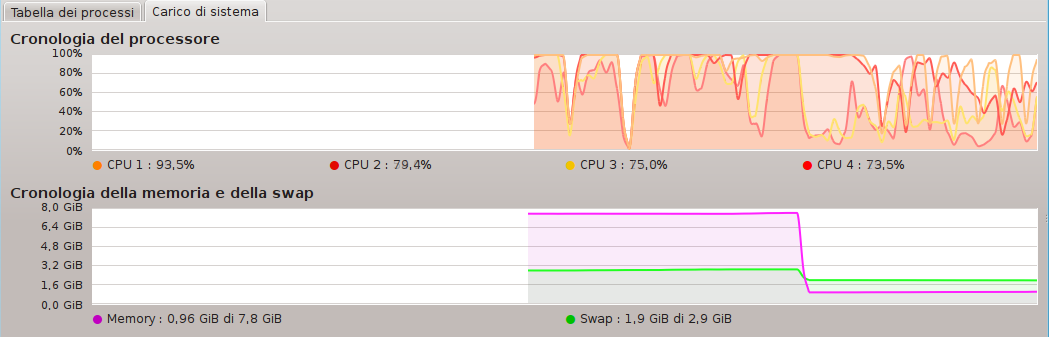
\includegraphics[width=1.0\textwidth]{assets/sib-memory-leak.png}
	\caption{Memory Leak del SIB che avveniva quando la connessione viene interrotta da un socket-timeout}
	\label{fig:sib-memory-leak}
\end{figure}

\noindent
L'insorgere del problema ha richiesto l'ottimizzazione delle performance e ho quindi deciso di limitare il numero di risposte fornite dal servizio cittadino (Par. ~\ref{par:thread}) poiché causava un ingente traffico di dati da e verso il SIB. Un'altra ottimizzazione apportata in seguito al problema è stata la trasformazione di INSERT di triple in query SPARQL: grazie all'uso dei prefissi al posto degli URL interi, si è ottimizzato notevolmente il volume di dati scambiato, con notevoli vantaggi durante l'uso nell'applicazione mobile.









